\documentclass[9pt, aspectratio=169]{beamer}
\usepackage{FiraSans}
\usetheme{metropolis}
\usepackage[utf8]{inputenc}
\usepackage{amsmath}
\usepackage{amsfonts}
\usepackage{amssymb}
\usepackage{multicol}
\usepackage{tikz}
\usepackage[T1]{fontenc} 
\usepackage[skins]{tcolorbox}
\usepackage{animate}
\author{Nicola Roman\`o - nicola.romano@ed.ac.uk}
\title{Dealing with large datasets - Part 2}
\setlength{\fboxsep}{0pt}
\setbeamertemplate{caption}{\raggedright\insertcaption\par}
\setbeamertemplate {footline}{\begin{scriptsize}\hfill\insertframenumber ~of \inserttotalframenumber\kern1em\vskip5pt\end{scriptsize}}

%\setbeamercovered{transparent} 
%\setbeamertemplate{navigation symbols}{} 

\titlegraphic{\centering 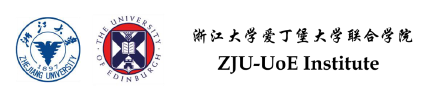
\includegraphics[scale=.5]{instituteLogo.png}}
%\institute{} 
\date{}
%\subject{} 

\begin{document}

\newtcolorbox{codebox}{enhanced,
	top=2pt,
	left=2pt,
	right=2pt,
	bottom=2pt,
	boxrule=0pt,
	leftrule=5pt,
	sharp corners,
	colback=gray!20,
	colframe=blue!60!black}

\begin{frame}
	\titlepage
\end{frame}

\begin{frame}
	{Last lecture we learned about...}
	\begin{itemize}
		\item Big data, and the problems associated with it!
		\item Using HDF5 file format to store and efficiently access big datatets.
	\end{itemize}
\end{frame}

\begin{frame}
	{Danger, too much data ahead!}
	\begin{columns}
		\begin{column}{.5\textwidth}
			\begin{figure}
				\centering
				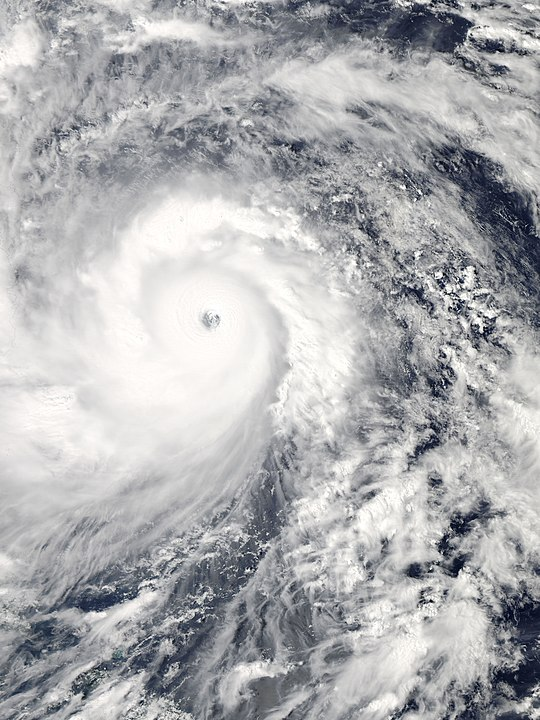
\includegraphics[width=.7\textwidth]{storm.jpg}
				\caption{\color{gray}{Souce: NASA, Public Domain}}
			\end{figure}
		\end{column}
		\begin{column}{.5\textwidth}
			\large
			How not to drown in a sea of [image] data?

			\vspace{1em}

			\normalsize
			Problem-dependent solutions, today we will focus on:

			\begin{itemize}
				\item Hardware solutions
				\item Choice of file format
				\item Parallelization
				\item Lazy evaluation/loading
				\item \dots
			\end{itemize}
		\end{column}
	\end{columns}
\end{frame}

\begin{frame}
	{Learning objectives}
	At the end of this lecture you should be able to:
	\begin{itemize}
		\item Describe the concept of parallelization
		\item Implement simple parallelization in Python
		\item Use dask to access larger-than-memory arrays in Python
		\item Use dask to perform delayed computation
	\end{itemize}
\end{frame}

\begin{frame}
	{Parallelization}
	Improving computer specifics is not always possible and is not necessarily the best solution.\\
	\vspace{2em}
	\begin{columns}
		\begin{column}{.4\textwidth}
			Imagine having three tasks to perform\\
			\vspace{2em}
			\centering
			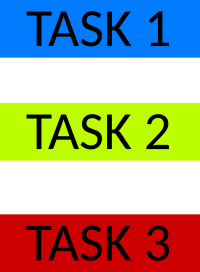
\includegraphics[width=.3\textwidth]{threetasks.png}
		\end{column}
		\pause
		\begin{column}{.6\textwidth}
			We can perform the tasks in different ways\\
			\vspace{2em}
			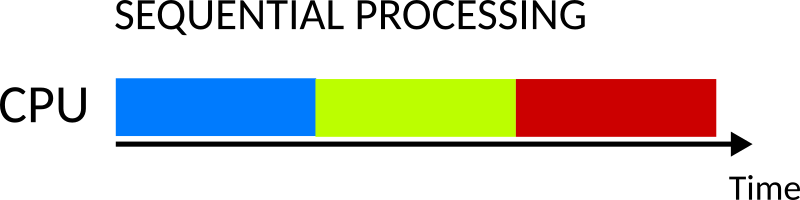
\includegraphics[width=.65\textwidth]{sequential.png}\\
			\pause
			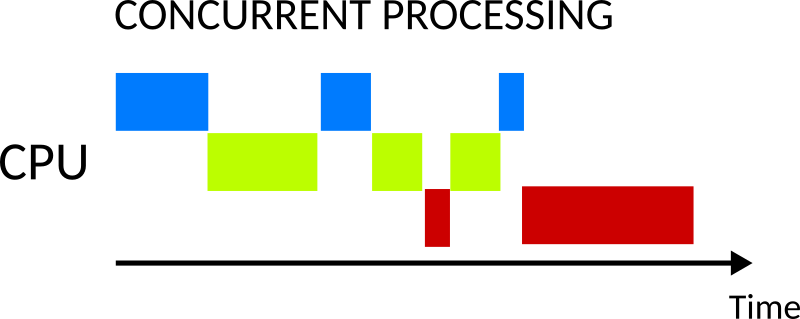
\includegraphics[width=.65\textwidth]{concurrent.png}\\
			\pause
			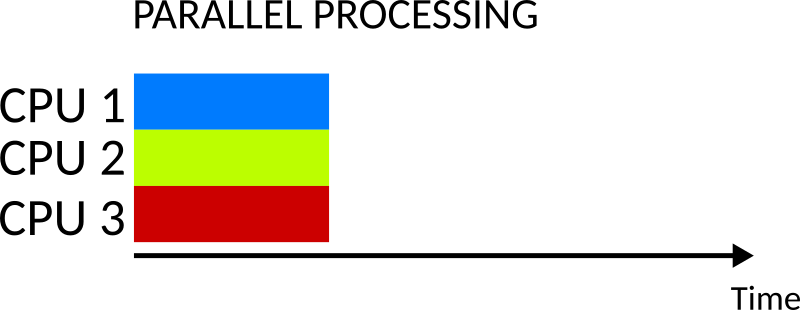
\includegraphics[width=.65\textwidth]{parallel.png}
		\end{column}
	\end{columns}
\end{frame}

\begin{frame}
	{Sequential, concurrent, and parallel processing}

	A few considerations on different processing modalities.

	\begin{itemize}
		\item Concurrent processing can only work if the tasks are \textbf{independent}.
		\item If task 3 depends on the output of task 2, which depends on the output of task 1, then you need to execute them sequentially.
		\item Concurrent processing can be faster than sequential, even on a single processor, for example if tasks need to wait for data.
		\item Remember that there is a (small) overhead in switching between "tasks"
	\end{itemize}
\end{frame}

\begin{frame}
	{Threads and processes}
	\begin{itemize}
		\item A \textbf{process} is the instance of a computer program executed by the operating system.
		\item A process can "spawn" multiple \textbf{threads}, each of which can execute an independent operation.
		\item Processes don't share memory space, while threads do.
		      \pause
		\item To avoid \textit{race conditions}, where multiple threads can modify the same data at the same time, Python implements a \textbf{Global Interpreter Lock} (GIL), which prevents threads to run at the same time
		\item The GIL makes python \textit{thread safe}, but does not allow running threads on multiple processors.
		      \pause
		\item Processes are not affected by GIL.
	\end{itemize}
\end{frame}

\begin{frame}
	{Threads and processes in Python}

	\begin{itemize}
		\item Use the \textit{multiprocessing} module to create processes
		\item Use the \textit{threading} module for threads or alternatively the \textit{multiprocessing.dummy} module.
		\item \textit{multiprocessing.dummy} is useful as it allows you to use the same exact code for creating processes but it creates threads instead!
		\item More examples in the practical!
	\end{itemize}
\end{frame}

\begin{frame}
	{Sequential execution}
	We execute a slow function sequentially
	\begin{codebox}
		\texttt{from time import sleep\\
		\\
		def slow\_function(n):\\
		$~~~~$\# This stops execution for 1 second\\
		$~~~~$sleep(1)\\
		return n*n\\
		\\
		result = [slow\_function(i) for i in range(4)]\\
		print(result)}
	\end{codebox}

	This takes (on my laptop with 4 cores) 4s and returns [0, 1, 4, 9]
\end{frame}

\begin{frame}
	{Parallel execution}
	We execute a slow function in parallel

	\begin{codebox}
		\texttt{import multiprocessing as mp\\			
			\\
			\# Start a "pool" of processes holding a maximum of\\
			\# processes equal to the number of CPU cores\\
			pool = mp.Pool(mp.cpu\_count())\\
			\\
			result = pool.map(slow\_function, range(4))\\
			pool.close()\\
			pool.join()\\
			print(result)
		}
	\end{codebox}

	\only<3->{This takes (on my laptop with 4 cores) 1.17s and still returns [0, 1, 4, 9] (luckily!). Note that processes may finish in different order, but that does not affect the order of the output!}
\end{frame}

\begin{frame}{Clean up the pool!}
	What does this mean, at the end of the previous piece of code?
	\begin{codebox}
		\texttt{pool.close()\\
			pool.join()}
	\end{codebox}
	\pause
	\begin{itemize}
		\item Pools are reusable.
		\item You could call \texttt{pool.map} again on the same pool.
		      \pause
		\item You should call \texttt{pool.close()} when you are done with the pool.
		\item \texttt{pool.close} prevents any more tasks from being submitted to the pool.
		      \pause
		\item \texttt{pool.join} should be called \textbf{after} \texttt{pool.close}
		\item \texttt{pool.join} makes the pool wait until all tasks are completed then exits.
	\end{itemize}
\end{frame}
\begin{frame}
	{Dealing with larger than memory arrays}
	\centering
	
\includegraphics[width=0.2\textwidth]{dask.png}

	Consider a case when you wanted to load several large images in memory, 3Gb each. \\
	It is likely that you won't be able to load such a large amount of data all at once.

	The \textit{dask} Pyton library helps solving this problem!\\
	\pause
	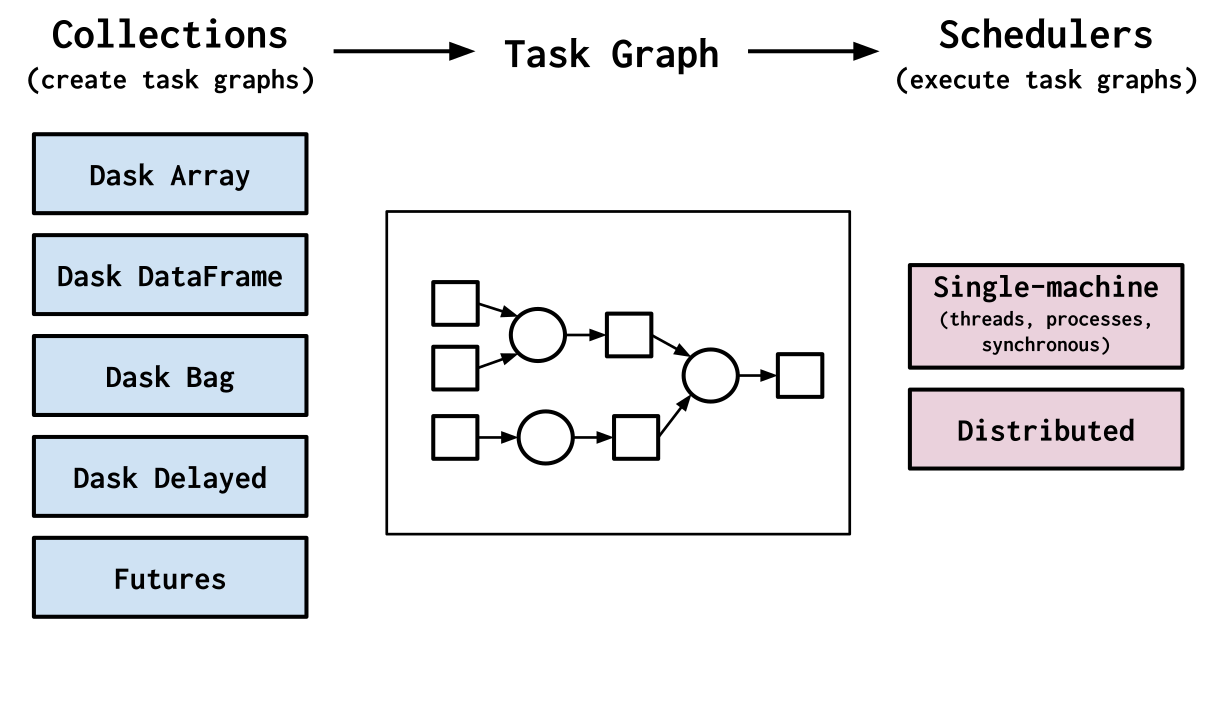
\includegraphics[width=.7\textwidth]{dask-overview.png}
\end{frame}

\begin{frame}
	{Delaying operation}
	\begin{codebox}
		\texttt{from dask import delayed\\
			\\
			def slow\_function(n):\\
			$~~~~$\# This stops execution for 5 seconds\\
			$~~~~$sleep(1)\\
			$~~~~$return n * n\\
			\\
			result = delayed(slow\_function)(1)
		}
	\end{codebox}
	\pause
	This takes 1.4 ms as the code \textbf{is not executed}.\\
	To effectively perform the operation we use

	\begin{codebox}
		\texttt{result.compute()}
	\end{codebox}

	Which now takes 1 second to run.
\end{frame}
\begin{frame}
	{Task graphs}
	Dask puts operations in a task graphs and executes them in an optimised way when needed.
	\begin{columns}
		\begin{column}{.6\textwidth}
			\begin{codebox}
				\texttt{def inc(x):\\
					$~~~~$sleep(1)\\
					$~~~~$return x + 1\\
					\\
					def add(x, y):\\
					$~~~~$sleep(1)\\
					$~~~~$return x + y\\
					\\
					x = delayed(inc)(1)\\
					y = delayed(inc)(2)\\
					z = delayed(add)(x, y)}
			\end{codebox}
			\pause
			This takes <1ms to run. Only once we run
			\begin{codebox}
				\texttt{z.compute()}
			\end{codebox}
			The calculation is performed, and takes 2 seconds
		\end{column}
		\begin{column}{.4\textwidth}
			\begin{figure}
				\pause
				\centering
				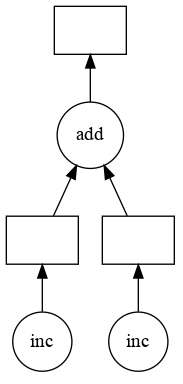
\includegraphics[width=.4\textwidth]{DAG.png}
				\caption{\centering Task graph can be visualized using \texttt{z.visualize("output.png")}}
			\end{figure}
		\end{column}
	\end{columns}
\end{frame}

\begin{frame}
	{The dask array container}
	You have a 1000-frame long video, and want to calculate the mean value every 10th frame\\
	\vspace{2em}
	\begin{columns}
		\begin{column}[t]{0.5\textwidth}
			\textbf{Numpy}\\
			~\\
			\begin{codebox}
				\texttt{import numpy as np\\
					x = np.random.randint(0, 255,\\
					$~~~$size=(1000, 1024, 1024))\\
					y = x[::10].mean()
				}
			\end{codebox}
			\only<2>{
				Runs in 12.8 s
			}
		\end{column}
		\begin{column}[t]{0.5\textwidth}
			\textbf{Dask}\\
			~\\
			\begin{codebox}
				\texttt{import numpy as np\\
					import dask.array as da\\
					\\
					\# ~1 billion elements\\
					x = da.random.randint(0, 255,\\
					$~~~$size=(1000, 1024, 1024),\\
					$~~~$chunks=(100, 64, 64))\\
					y = x[::10].mean()
				}
			\end{codebox}
			\only<2>{
				Runs in 0.55 seconds

				\begin{codebox}
					\texttt{y.compute()}
				\end{codebox}
				Runs in 3.66 s
			}
		\end{column}
	\end{columns}
\end{frame}

\begin{frame}{What's happening under the hood...}
	\begin{figure}
		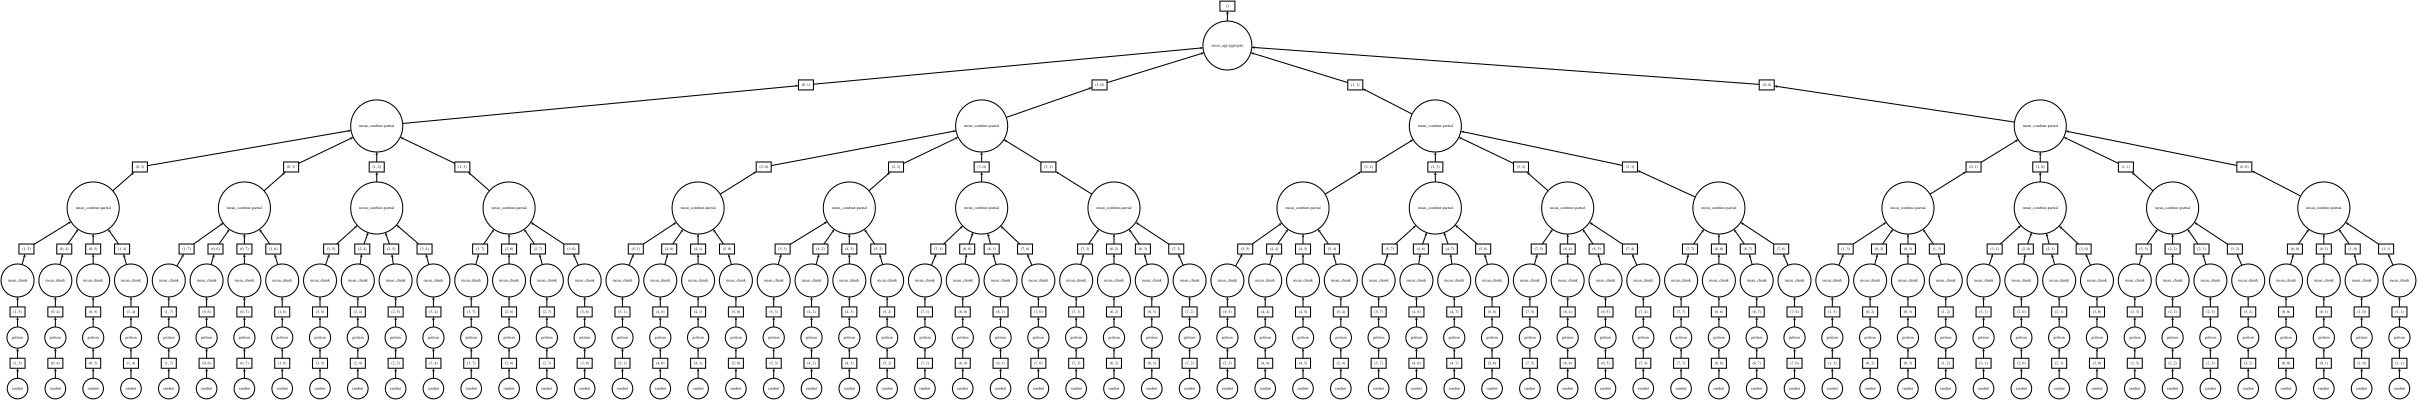
\includegraphics[width=\textwidth]{biggraph.png}
		\caption{No, you're not supposed to be able to read this image...}
	\end{figure}
	\pause
	\begin{itemize}
		\item Dask is splitting your task into many subtasks
		      \begin{itemize}
			      \item Generate a subset of the random numbers
			      \item Calculate partial means
			      \item Pulling those means together
			      \item Pulling those new means together
			      \item \dots
			      \item Get the final value!
		      \end{itemize}
		      \pause
		\item Subtasks can run on different CPUs/GPUs, even on different computers!
		\item Subtasks will run from bottom to top, but may run in any left/right order.
		\item These are simpler and faster to handle and fit into memory
	\end{itemize}
\end{frame}

\begin{frame}
	{Delayed loading of images with Dask}
	Let's delay imread
	\begin{columns}
		\begin{column}{.5\textwidth}
			\begin{codebox}
				\texttt{from skimage.io import imread\\
				from dask import delayed\\
				\\
				\# 1500 images of a 2048x2048 movie\\
				filenames = [f"images/image\{i:04d\}.tif"\\
				$~~~~$for i in range(1500)]\\
				delayed\_img = [delayed(imread)(fn)\\
				$~~~~$for fn in filenames]\\
				dask\_arrays = [da.from\_delayed(im,\\
				$~~~~$shape=(2048, 2048), dtype=np.uint8)\\
				$~~~~$for im in delayed\_img]\\
				\pause
				stack = da.stack(dask\_arrays, axis=0)\\
				\# We can also modify chunk size\\
				stack = stack.rechunk((10, 512, 512))}
			\end{codebox}
		\end{column}
		\begin{column}{.5\textwidth}
			\only<2>{
				\centering
				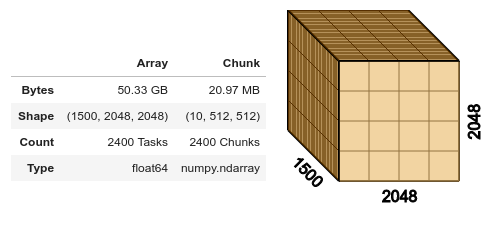
\includegraphics[width=\textwidth]{stack.png}}
		\end{column}
	\end{columns}
\end{frame}

\begin{frame}
	{I/O on HDF5 files with Dask}
	\only<1>{You have an HDF file with the following structure\\
		\texttt{|\\
			|--> Control   |-> Experiment 1\\
			|$~~~~~~~~~~~$|-> Experiment 2\\
			|$~~~~~~~~~~~$|-> \dots\\
			|\\
			|--> Treatment |-> Experiment 1\\
			$~~~~~~~~~~~~~~$|-> Experiment 2\\
			$~~~~~~~~~~~~~~$|-> \dots}
	}
	\only<2->{You can read all the experiments using
		\begin{codebox}
			\texttt{import numpy as np\\
			import dask.array as da\\
			controls = [h5py.File("experiments.h5", "r")[f"/Control/Experiment {i}"]\\
			$~~~~$for i in np.arange(1, 10)]\\
			control\_data = [da.from\_array(c, chunks=(10, 128, 128))\\
			$~~~~$for c in controls]}
		\end{codebox}
		All experiments are loaded lazily, so this takes only a few ms to run.\\
		Data can be accessed rapidly and in parallel through dask only when needed.
	}
\end{frame}
\begin{frame}
	{Summary}
	\begin{itemize}
		\item We have only seen the tip of the iceberg.
		\item Big datasets are becoming ever more common and easy to access
		\item Think in advance about the challenges these data present and the strategies to overcome them
		\item Parallel processing can help greatly speed up your computations (even more when using GPUs)
		\item Chunked storage and processing of big arrays (or other data types), e.g. using dask, is an efficient way of dealing with large datasets
	\end{itemize}
	
\end{frame}
\end{document}